\documentclass[11pt,a4paper]{article}

% ==============================================================================
% HOJA DE ESTILOS DEL PROYECTO (estilos, paquetes, márgenes y encabezados)
% ==============================================================================
\usepackage{estilo_pericial}

% ==============================================================================
% METADATOS Y VARIABLES CONFIGURABLES DEL INFORME
% (Modifica estos valores una única vez para actualizar todo el documento)
% ==============================================================================
\renewcommand{\TituloInforme}{Informe Técnico Pericial}
\renewcommand{\SubtituloDocumento}{DICTAMEN PERICIAL}
\renewcommand{\Cliente}{EMPRESA SL}
\renewcommand{\Referencia}{ITP26-GP08}
\renewcommand{\FechaInforme}{19 de Novimebre de 2026}
\renewcommand{\CiudadFirma}{Valladolid}
\renewcommand{\FechaFirma}{24 de Noviembre de 2026}



% ==============================================================================
% INICIO DEL DOCUMENTO
% ==============================================================================
\begin{document}

% ------------------------------------------------------------------------------
% PORTADA
% ------------------------------------------------------------------------------
\GenerarPortadaPericial

% ------------------------------------------------------------------------------
% TABLA DE CONTENIDOS
% ------------------------------------------------------------------------------
\newpage
\tableofcontents
\newpage

% ------------------------------------------------------------------------------
% CUERPO DEL DICTAMEN PERICIAL (CARPETA: capitulos/)
% ------------------------------------------------------------------------------
\begin{center}
    {\LARGE\bfseries\textcolor{AzulPericial}{\SubtituloDocumento}}
\end{center}
\vspace{0.5cm}

% Ajuste para que la numeración comience en 0 (0. Resumen ejecutivo)
\setcounter{section}{-1}

\section{Resumen ejecutivo}

Tal y como se expondrá en el presente informe, en opinión de este perito, el análisis \ldots\ldots\ldots\ldots\ldots

A juicio de este perito \ldots\ldots\ldots\ldots\ldots

A juicio de este perito \ldots\ldots\ldots\ldots cuyo detalle se indica en el presente informe\ldots\ldots

Una vez analizado \ldots\ldots\ldots\ldots\ldots este perito estima que \ldots\ldots\ldots

\newpage

\section{Introducción}

\subsection{Sobre el Objeto del Peritaje}

A requerimiento de \textbf{\Cliente} se procede a la revisión de la filtración del fichero \textit{Condifencial.pdf}

Considerando los hechos y circunstancias anteriores, el Perito autor del presente informe técnico, de conformidad con lo dispuesto por el artículo 335.2 de la Ley de Enjuiciamiento Civil, quiere hacer las siguientes manifestaciones:

\begin{itemize}[leftmargin=1.5em]
    \item El presente dictamen lo emite bajo promesa de decir la verdad.
    \item Ha actuado con la mayor objetividad posible, tomando en consideración tanto lo que pueda favorecer como lo que sea susceptible de causar perjuicio a cualquiera de las partes.
    \item El perito manifiesta su total imparcialidad y la no concurrencia de ninguna de las circunstancias por las que poder ser objeto de tachas, recogidas en el artículo 343 de la Ley de Enjuiciamiento Civil:
    \begin{enumerate}[label=\alph*), leftmargin=1.8em]
        \item Ser cónyuge o pariente por consanguinidad o afinidad, dentro del cuarto grado civil de una de las partes o de sus abogados o procuradores.
        \item Tener interés directo o indirecto en el asunto o en otro semejante.
        \item Estar o haber estado en situación de dependencia o de comunidad o contraposición de intereses con alguna de las partes o con sus abogados o procuradores.
        \item Amistad íntima o enemistad con cualquiera de las partes o sus procuradores o abogados.
        \item Cualquier otra circunstancia, debidamente acreditada, que les haga desmerecer en el concepto profesional.
    \end{enumerate}
\end{itemize}

\subsection{Sobre el Perito}

\subsection{Sobre los Peritos}

El presente dictamen ha sido elaborado conjuntamente por los siguientes integrantes del \textbf{\GrupoPracticas}:

\vspace{0.2cm}
\begin{sloppypar}
	\textbf{\PeritoUno.} Colegiado n.\textsuperscript{o} \NumColegiadoUno\ del \ColegioProfesional\ (\url{\WebColegio}), es Licenciado e Ingeniero / Máster en Informática por la \UniversidadPerito.
\end{sloppypar}

Profesionalmente, desempeña su actividad principal como desarrollador de \textit{software}

Ha recibido formación como perito por parte del \ColegioProfesional\ y por parte de Universidad de Valladolid.

Ha realizado peritajes similares a este, en el ámbito de los sistemas de información.

\vspace{0.3cm}
\begin{sloppypar}
	\textbf{\PeritoDos.} Colegiado n.\textsuperscript{o} \NumColegiadoDos\ del \ColegioProfesional\ (\url{\WebColegio}), es Licenciado e Ingeniero / Máster en Informática por la \UniversidadPerito.
\end{sloppypar}

Profesionalmente, desempeña su actividad principal como desarrollador de \textit{Software}

Ha recibido formación como perito por parte del \ColegioProfesional\ y por parte de la Universidad de Valladolid 

Ha realizado peritajes similares a este, en el ámbito de los sistemas de información.

\vspace{0.3cm}
\begin{sloppypar}
	\textbf{\PeritoTres.} Colegiado n.\textsuperscript{o} \NumColegiadoTres\ del \ColegioProfesional\ (\url{\WebColegio}), es Licenciado e Ingeniero / Máster en Informática por la \UniversidadPerito.
\end{sloppypar}

Profesionalmente, desempeña su actividad principal como estudiante de ingeniería informática

Ha recibido formación como perito por parte del \ColegioProfesional\ y por parte de la Universidad de Valladolid.

Ha realizado peritajes similares a este, en el ámbito de los sistemas de información.

\vspace{0.3cm}
\begin{sloppypar}
	\textbf{\PeritoCuatro.} Colegiado n.\textsuperscript{o} \NumColegiadoCuatro\ del \ColegioProfesional\ (\url{\WebColegio}), es Licenciado e Ingeniero / Máster en Informática por la \UniversidadPerito.
\end{sloppypar}

Profesionalmente, desempeña su actividad principal como estudiante de ingeniería informática.

Ha recibido formación como perito por parte del \ColegioProfesional\ y por parte de la Universidad de Valladolid.

Ha realizado peritajes similares a este, en el ámbito de los sistemas de información.

\newpage

\section{Consideraciones generales}

\subsection{Sobre los servidores Windows y los registros de eventos.}
En los sistemas operativos para servidores de la familia Microsoft Windows, y de forma específica en \textbf{Windows Server 2008 R2}, la trazabilidad de la actividad del sistema se gestiona mediante la arquitectura \textit{Windows Event Log}. Dichos registros se almacenan en formato binario estructurado basado en XML con extensión \texttt{.evtx}, ubicados por defecto en el directorio protegido del sistema \texttt{C:\textbackslash Windows\textbackslash System32\textbackslash winevt\textbackslash Logs\textbackslash}. De tal manera que el resgitro de las acciones realizadas sobre el servidor se almacenan en binario y necesitamos un programa concreto para traducirlo a un texto legible por el humano.

El sistema clasifica las entradas en registros principales (\textit{Aplicación}, \textit{Seguridad}, \textit{Sistema} e \textit{Instalación}) y registros operativos específicos. Cada evento incorpora de forma estructurada un identificador numérico (\textit{Event ID}), la marca temporal exacta (almacenada internamente en formato UTC(formato estándar para el tratamiento del formato horario en los dispositivos)), el origen del evento, el nivel de gravedad, el equipo y el identificador de seguridad (\texttt{<SID>}) del usuario asociado. Desde el punto de vista pericial, estos registros constituyen una fuente primaria de auditoría que permite reconstruir cronológicamente inicios de sesión, accesos a recursos, ejecuciones de servicios y modificaciones de configuración, siempre que se verifique la integridad de los ficheros de registro y la sincronización horaria del servidor.

\subsection{Sobre las cabeceras de un correo electrónico.}
En las comunicaciones mediante correo electrónico basadas en el protocolo SMTP (estándar para la creación de mails y el estándar \href{RFC 5322}{https://www.rfc-editor.org/info/rfc5322/}(estándar del intercambio de mensajes a través de la re), todo mensaje se compone de un cuerpo y un bloque de cabeceras (\textit{headers}) que documentan su tránsito desde el origen hasta el destino. Las cabeceras contienen metadatos(grupo de datos que describen el contenido informativo de, en este caso, el correo) de enrutamiento (líneas \texttt{Received} añadidas secuencialmente en orden cronológico inverso por cada servidor de correo intermediario), direcciones de remitente y destinatario (\texttt{From}, \texttt{To}, \texttt{Return-Path}), un identificador único de mensaje (\texttt{Message-ID}), marcas temporales y resultados de validación criptográfica y de dominio siguiento los siguientes protocolos:
\begin{itemize}
	\item \texttt{SPF(\textit{Sender Policy Framework}}: lista de control de acceso publicada en los registros DNS (\textit{Domain Name System}) de un dominio donde el propietario indica qué direcciones IP (\textit{Internet Protocolo}) o servidores están autorizados para enviar correos en su nombre. En un lenguaje menos técnico, permite establecer una lista de qué personas o empresas pueden enviar un correo.
	\item  \texttt{DKIM(\textit{DomainKeys Identified Mail})}: añade una firma criptográfica digital en la cabecera del correo (\textit{DKIM-Signature}) generada con una clave privada que solo posee el servidor de salida del remitente. Añadiendo unas capas de seguridad extra, puesto que el cifrado de la comunicación emplea un mecanismo para cifrar el mensaje en tránsito y solo las persoans autorizadas pueden desencriptarlos.
	\item  \texttt{DMARC}(\textit{Domain-based Message Authentication, Reporting, and Conformance}): capa de políticas que coordina a SPF y DKIM. Exige que exista \textbf{alineación} (que el dominio visible para el usuario en el campo From: coincida con el dominio validado por SPF o DKIM) e indica al servidor receptor cómo actuar si ambos fallan.
\end{itemize}

A efectos probatorios, si bien los campos visibles en el cliente de correo (como el remitente aparente o la fecha local) son susceptibles de alteración, el análisis forense de la cadena completa de campos \texttt{Received}, las direcciones IP de los servidores intervinientes y los registros de autenticación del servidor permiten acreditar técnicamente el origen real, la ruta de transmisión y la integridad temporal del envío.

\subsection{Sobre la aplicación Dropbox y su sincronización con la nube.}
Para comprender el funcionamiento de la plataforma de almacenamiento en la nube Dropbox en entornos Windows, debe distinguirse entre el repositorio remoto en servidores del proveedor y el cliente local instalado en el equipo. El cliente sincroniza de forma automatizada una carpeta local del sistema de ficheros con la cuenta vinculada en la nube, registrando cada operación de creación, modificación, renombrado o eliminación de archivos.

A nivel forense, el cliente mantiene bases de datos locales de caché y configuración (como \texttt{filecache.dbx} o \texttt{config.dbx}) en el perfil del usuario, mientras que la plataforma remota conserva un historial de revisiones, marcas temporales de sincronización y registros de conexión (incluyendo direcciones IP y dispositivos vinculados). La correlación entre los artefactos locales del servidor y los registros de actividad de la cuenta permite establecer la trazabilidad y causalidad de las operaciones realizadas sobre los documentos sincronizados.

\subsection{Sobre el borrado de ficheros en Windows y la papelera de reciclaje.}
Para analizar la eliminación de información en \textbf{Windows Server 2008 R2}, es preciso atender al funcionamiento del sistema de archivos \textbf{NTFS} (\textit{New Technology File System}), el cual indexa cada fichero y directorio mediante registros en la Tabla Maestra de Archivos (\texttt{\$MFT}). Cuando un usuario realiza un borrado lógico en Windows, pueden producirse dos escenarios técnicamente diferenciados:

\begin{itemize}[leftmargin=1.5em]
	\item \textbf{Eliminación estándar (envío a la Papelera de Reciclaje):} El fichero no se destruye, sino que se traslada al directorio oculto del sistema \texttt{C:\textbackslash \$Recycle.Bin\textbackslash <SID>\textbackslash}, segregado por el identificador de seguridad único (\texttt{<SID>}) de cada cuenta de usuario. En dicha ubicación se generan dos artefactos: un fichero de metadatos con prefijo \texttt{\$I} (que conserva la ruta original, el tamaño y la marca temporal exacta del borrado) y un fichero con prefijo \texttt{\$R} que contiene los datos íntegros del archivo.
	\item \textbf{Eliminación permanente (\texttt{Shift + Supr}, vaciado de papelera o borrado mediante consola):} El sistema operativo marca el registro correspondiente de la \texttt{\$MFT} como disponible y libera los clústeres asignados en el mapa de bits del volumen (\texttt{\$Bitmap}), dejando el espacio como no asignado (\textit{unallocated space}) sin sobrescribir de inmediato el contenido binario en el soporte físico.
\end{itemize}

\newpage
\subsection{Sobre el borrado de ficheros en Windows y la papelera de reciclaje.}
Para analizar la eliminación de información en \textbf{Windows 11}, es preciso atender al funcionamiento del sistema de archivos \textbf{NTFS} (\textit{New Technology File System}), el cual indexa cada fichero y directorio mediante registros en la Tabla Maestra de Archivos (\texttt{\$MFT}). Cuando un usuario realiza un borrado lógico en Windows 11, pueden producirse dos escenarios técnicamente diferenciados:

\begin{itemize}[leftmargin=1.5em]
	\item \textbf{Eliminación estándar (envío a la Papelera de Reciclaje):} El fichero no se destruye, sino que se traslada al directorio oculto del sistema \texttt{C:\textbackslash \$Recycle.Bin\textbackslash <SID>\textbackslash}, segregado por el identificador de seguridad único (\texttt{<SID>}) de cada cuenta de usuario. En dicha ubicación se generan dos artefactos: un fichero de metadatos con prefijo \texttt{\$I} (que conserva la ruta original en formato Unicode, el tamaño y la marca temporal exacta del borrado) y un fichero con prefijo \texttt{\$R} que contiene los datos íntegros del archivo. Asimismo, si las carpetas del perfil se encuentran sincronizadas con \textbf{OneDrive} (integrado de forma nativa en Windows 11), la eliminación se replica en la nube trasladando el archivo a la papelera de reciclaje en línea de la cuenta.
	\item \textbf{Eliminación permanente (\texttt{Shift + Supr}, vaciado de papelera o borrado mediante consola):} El sistema operativo marca el registro correspondiente de la \texttt{\$MFT} como disponible, registra la transacción en el diario de cambios (\texttt{\$UsnJrnl}) y libera los clústeres asignados en el mapa de bits del volumen (\texttt{\$Bitmap}), dejando el espacio como no asignado (\textit{unallocated space}). En unidades de almacenamiento magnéticas (HDD) o soportes externos, el contenido binario permanece sin sobrescribir de inmediato; no obstante, en unidades de estado sólido (\textbf{SSD/NVMe}), Windows 11 emite de forma predeterminada el comando \textbf{TRIM} hacia la controladora del disco para optimizar el rendimiento, lo que puede provocar el borrado físico o desasignación inmediata de los bloques liberados.
\end{itemize}

\subsection{Sobre la recuperación de ficheros borrados en Windows}
Para proceder a la recuperación forense de archivos eliminados en sistemas \textbf{Windows 11}, debe evaluarse tanto la persistencia lógica en el sistema de archivos NTFS como la naturaleza física del soporte de almacenamiento (HDD frente a SSD con soporte \textit{TRIM}), no es lo mismo un disco magnético, como es el HDD a uno que hace la lectura por láser como el SSD y el estado del cifrado de dispositivo (\textbf{BitLocker}, habitualmente activo por defecto en equipos modernos con Windows 11) puesto que es un herramienta de Microsoft que cifra el disco en caso de detectar una actividad sospechosa sobre el mismo.

Cuando los bloques de datos no han sido sobrescritos ni purgados mediante \textit{TRIM}, la recuperación se lleva a cabo mediante técnicas de análisis de registros residuales de la \texttt{\$MFT} y del diario \texttt{\$UsnJrnl}, búsqueda por firmas de cabecera y pie de archivo en el espacio no asignado (\textit{file carving}), extracción desde instantáneas de volumen (\textit{Volume Shadow Copies} o puntos de restauración del sistema, siempre que la Protección del Sistema se encuentre habilitada en el volumen) o recuperación desde el historial de versiones y papelera remota de OneDrive. Con el fin de preservar la cadena de custodia y garantizar la validez legal de los hallazgos, toda operación de adquisición, descifrado y recuperación debe ejecutarse exclusivamente sobre una copia o imagen forense previamente verificada mediante funciones resumen criptográficas, manteniendo el soporte original inalterado.
\newpage
\subsection{Sobre los registros de log}
Todo sistema de información dispone de una serie de registros en los cuales quedan registradas todas las actividades y actuaciones que realiza el sistema, así como todos los errores que se producen al intentar realizar las diferentes tareas que tiene programadas. Estos registros se pueden almacenar en base de datos o en un fichero en el servidor.

%\subsection{Sobre la aplicación Whatsapp}
%La aplicación WhatsApp almacena sus contenidos dentro del dispositivo y estos son trasladados a la copia de seguridad que se realiza diariamente sobre el propio dispositivo.
%
%Esta copia de seguridad se almacena en la carpeta del dispositivo con nombre \texttt{Whatsapp/Databases} en diferentes ficheros con el formato ``\texttt{msgstore*.db.crypt12}''.
%
%La propia aplicación dispone de una opción llamada ``Enviar chat por correo'' que envía por correo electrónico todo el contenido de una conversación.
%
%\subsection{Sobre la conexión de dispositivos Samsung}
%Los dispositivos Samsung permiten navegar por las carpetas del dispositivo una vez que se conecta a un ordenador autorizado. Esta navegación se realiza en modo solo lectura utilizando la aplicación ``USB Write Blocker'' para evitar toda manipulación en el dispositivo.
%
%Mediante esta conexión de SOLO LECTURA se extraen las copias de seguridad almacenadas en la carpeta del dispositivo con nombre \texttt{Whatsapp/Databases} en diferentes ficheros. También mediante esta conexión de SOLO LECTURA se extraen varios ficheros de audio en formato MP3.
%
%Todos los ficheros, una vez creado su código HASH, se almacenan en un dispositivo USB con número de serie ``\texttt{xxxxxxxxxxxxxxxxxxxxx}'' que se presenta como evidencia.

\subsection{Sobre las funciones de resumen HASH.}
Los hash o funciones de resumen son algoritmos que consiguen crear a partir de una entrada (ya sea un texto, una contraseña o un archivo, por ejemplo) una salida alfanumérica de longitud normalmente fija que representa un resumen de toda la información que se le ha dado (es decir, a partir de los datos de la entrada crea una cadena que solo puede volverse a crear con esos mismos datos). Para la realización de este peritaje se ha utilizado una función HASH SHA-1.
%
%\subsection{Sobre los SMS en iPhone}
%Los SMS en iPhone se almacenan en el propio dispositivo y estos son trasladados a la copia de seguridad que se realiza con iTunes.
%
%\subsection{Sobre la herramienta iTunes}
%Se trata de una herramienta propia de Apple que sirve para realizar copias de seguridad de los dispositivos iPhone, entre otros. La copia de seguridad se realiza de manera que el dispositivo no se modifica en ningún momento.
%
%\subsection{Sobre la herramienta iPhone Backup Extractor}
%Se trata de una herramienta de la empresa Reincubate para analizar el backup de un dispositivo iPhone y extraer de forma segura su contenido sin modificar la fuente original de la información.
%
%Recupera todas tus fotos perdidas, Photostream, mensajes, SMS, videos, buzón de voz, notas, llamadas, chats de Whatsapp, contactos, entradas en el calendario y datos inaccesibles de otras aplicaciones.
%
%Funciona con las copias de seguridad de iPhone X, iPhone 8, 8 Plus, iPhone 7 Plus, iPhone 7, iPhone SE, 6 y 6S, iPhone 6 Plus y 6S Plus, iPhone 5, iPhone 5, iPhone 5c, iPhone 4, iPhone 3G, iPhone 3G, iPod, iPad de todas las versiones de iTunes, iCloud e iOS, incluido iOS 11 y 10.3.
%
%Entre los formatos de extracción que admite he extraído en PDF, HTML y CSV para los chat de Whatsapp y el VCF para los contactos.

\newpage

\section{Consideraciones específicas}

\subsection{Sobre el servidor de correo eléctronico}
	%% =====================================================================
% Capítulo: Servidor de correo para el Escenario 1 (fuga por correo)
% Se incluye desde el main con \include{servidor} (sin extensión).
%
% Todo el diseño sale de styles/mistilo.sty (que ya carga listings,
% booktabs, caption, float, xcolor, tcolorbox, etc.). Este capítulo solo
% usa lo que ese estilo define:
%   - listados:  style=terminal
%   - avisos:    entorno aviso
%   - tablas:    booktabs + caption
% Idioma y codificación los decide el main; hace falta:
%   \usepackage[T1]{fontenc}   % para que < y > salgan bien en \texttt
% =====================================================================

% Código en línea (admite _, $, ^, {}, <, > ... sin escapar)
\providecommand{\cod}[1]{\texttt{\detokenize{#1}}}

\subsection{Configuración del servidor de correo electrónico para el escenario de fuga de información por correo}
\label{cap:servidor}

El objetivo de este capítulo es explicar la creación del sistema de correo preparado para el primero de los escenarios detallados en el enunciado; si bien no entraremos en detalles muy técnicos, en caso de querer profundizar en el código fuente de la aplicación así como la información técnica y una guía de uso e instalación, se puede revisar en el \href{https://github.com/ALVPI/IFOR_P2/tree/main/servidor}{repositorio del grupo H} para esta práctica.


Para poder realizar este trabajo vamos a empler el protocolo SMPT según se especifica en el \href{https://www.rfc-editor.org/info/rfc5321/}{RFC 5321} adaptándolo para nuestro entorno el cual van a ser dos VMs (máquinas virtuales) con el sistema operativo Windows 11.
\section{Funcionalidades}
Nuestro sevidor de correo y por consecuencia su portal web tiene van a realizar las siguientes funcionalidades:
\begin{enumerate}
  \item permita enviar \cod{Confidencial.pdf} como adjunto entre dos buzones
        del grupo \cod{pepe@empresa.local} $\rightarrow$
        \cod{ana@empresa.local}; los dos usuarios por defecto que hemos creado en el propio servidor.
  \item dejare \textbf{evidencia analizable} en disco (\cod{.eml} completo con
        cabecera \cod{Received}, adjunto extraído, log de auditoría);
\end{enumerate}
% ---------------------------------------------------------------------
\subsection{Decisiones técnicas y por qué}
Una vez tenemos claro cuál es el objetivo a cumplir, hemos tenido que tomar una serie de decisiones sobre el \textit{stack} tecnológico, es decir, protocolos, leguajes, librerias que vamos a emplear siguiendo lo especificado en el RFC correspondiente 
\begin{table}[H]
\centering
\small
\renewcommand{\arraystretch}{1.3}
\begin{tabular}{@{}p{0.32\textwidth}p{0.64\textwidth}@{}}
\toprule
\textbf{Decisión} & \textbf{Motivo} \\
\midrule
\textbf{Python 3, solo stdlib} (sin \cod{pip}) &
En las VMs no hay internet garantizado; \cod{socket}, \cod{email} y
\cod{http.server} bastan. Se arranca con \cod{py -3 servidor.py} en Windows. \\
\textbf{SMTP desde cero} (RFC 5321) &
Es lo didáctico y lo evaluado: HELO/EHLO, MAIL, RCPT, DATA y los códigos
2xx/4xx/5xx. Una librería (\cod{aiosmtpd}) ocultaría el protocolo. \\
\textbf{Webmail con \cod{http.server}} &
Cubre lo esencial de un <<Gmail>> (bandeja, leer, descargar adjuntos,
redactar) sin Flask ni dependencias. \\
\textbf{Sin autenticación} &
Para simplificar la complejidad de este ejercicio, como estamos en un entorno simulado hemos decidido \textbf{no} implementar un sistema de autenticación. \\
\textbf{Servidor en una VM Win10/11 dedicada} &
Puertos 25 (SMTP) y 8080 (webmail) en la red NAT de VirtualBox ya
configurada. \\
\textbf{Almacenamiento en ficheros} &
\cod{buzones/<usuario>/mensajes/*.eml} + \cod{adjuntos/} extraídos: fácil de
inspeccionar como evidencia. \\
\textbf{Pruebas con \cod{unittest}} (stdlib) &
Para verificar que el sistema funcionad e manera correcta.\\
\bottomrule
\end{tabular}
\caption{Decisiones técnicas del servidor de correo.}
\label{tab:decisiones-servidor}
\end{table}


% ---------------------------------------------------------------------
\subsection{Almacenamiento  de Logs y evidencias (cadena de custodia)}
Una vez hemos expuesto las decisiones de diseño de nuestro servidor vamos a detaller como funciona el registro de correos, ya que es la parte más importante del sistema para poder sacar conclusiones en un proceso de peritaje informático.\\

\begin{itemize}
  \item Cada mensaje se guarda como \textbf{\cod{.eml}} (mensaje MIME completo
        con todas las cabeceras, incluida \cod{Received} con la IP de origen,
        el HELO y la fecha).
  \item Los \textbf{adjuntos se extraen} a una carpeta por mensaje, con
        nombres saneados, de modo que un \cod{.pdf} se abre sin parsear el
        \cod{.eml}.
  \item El identificador de cola (\cod{cola\_id}) tiene resolución de segundo +
        UUID (\textit{Universally Unique Identifier}), el identificador único de cada correo.
  \item \cod{usuarios.json} guarda la lista de buzones (el apartado donde se almacenan los coreos de cada usuario.) Siguiendo el siguiente formato(\cod{{"usuarios": [...]}}).
\end{itemize}

Con esto conseguimos que la evidencia se recopile \textbf{sin ser modificada} y queda lista para la cadena de custodia.

\subsubsection{Ejemplo de registro (\textit{log}) de un envío de correo}
\begin{lstlisting}[style=terminal,breaklines=true]
	2026-11-05T10:00:00 | de: pepe@empresa.local | para: ana@empresa.local, luis@empresa.local | asunto: Examen final | adjuntos: Confidencial.pdf (123 KB), notas.txt (4 KB)
\end{lstlisting}

Como podemos ver cada mensaje entregado, ya sea por \textbf{SMTP o por el webmail}, añade \textbf{una única línea} a \cod{logs/envios.log} (en lenguaje mundano, se guarda en la carpeta logs en el fichero envios.). 
Entendamos ahora un poco qué información nos proporciona este registro:
\begin{itemize}
	\item Timestamp \href{https://www.iso.org/standard/40130.html}{ISO 8601} en hora local (segundos).
	\item \cod{para}: destinatarios en el orden aceptado (RCPT TO / lista del
	formulario).
	\item \cod{adjuntos}: nombres saneados con tamaño redondeado a KB (mínimo
	1 KB); si no hay, \cod{adjuntos: ninguno}.
	\item \textbf{Escaping}: si el asunto o un nombre contiene \cod{ | } (o
	cualquier \cod{|}), se sustituye por \textbrokenbar{} (U+00A6), de
	modo que cada envío es \textbf{exactamente una línea} jamás rota.
	\item El fichero \textbf{crece por anexión} (nunca se reescribe); la
	escritura va protegida con lock y \cod{try/except}: un fallo del log
	(disco lleno, permisos\ldots) queda en el logger
	\cod{correo.log_envios} pero \textbf{nunca tumba} el envío ni la
	sesión.
\end{itemize}

% ---------------------------------------------------------------------
\subsection{Por qué esto se adapta al escenario de la fuga por correo}

\begin{enumerate}
  \item Arrancar \cod{todo} en la VM Win10/11 del servidor de correo.
  \item Crear dos buzones: \cod{pepe@empresa.local} y
        \cod{ana@empresa.local}.
  \item En el Windows Server 2008: enviar \cod{Confidencial.pdf} adjunto con
        cualquier cliente SMTP (o telnet/PowerShell) a
        \cod{ana@empresa.local}.
  \item Evidencias que quedan en el servidor:
        \begin{itemize}
          \item \cod{servidor/buzones/ana/mensajes/<id>.eml} --- mensaje
                completo con la cabecera \cod{Received} (origen, HELO,
                fecha);
          \item \cod{servidor/buzones/ana/adjuntos/<id>/Confidencial.pdf} ---
                el adjunto extraído, listo para imagen y cadena de custodia;
          \item \cod{servidor/logs/envios.log} --- línea de auditoría del
                envío.
        \end{itemize}
  \item En el webmail, bandeja de \cod{ana} $\rightarrow$ abrir $\rightarrow$
        descargar adjunto.
  \item Archivar todo (imágenes de disco) \textbf{sin modificar} y elaborar la
        cadena de custodia.
\end{enumerate}

Esto cubre exactamente lo que pide el enunciado: sacar \cod{Confidencial.pdf}
del Windows Server 2008, enviarlo por correo entre dos miembros del grupo y
conservar la evidencia analizable.


% ---------------------------------------------------------------------


\subsubsection{Sobre la fuga de información mediante el correo electrónico}
	%% =====================================================================
% Capítulo: Escenario 1 -- fuga de información mediante correo electrónico
% Misma estructura que el escenario USB (03_3_desarrollo_usb.tex):
% planteamiento, preparación, cadena de custodia, adquisición, análisis
% y conclusiones. Usa lo que define estilo_pericial.sty (listados con
% style=terminal y tablas con booktabs y caption).
%
% Los datos de la cadena de custodia proceden de los metadatos de los
% ficheros del propio laboratorio (carpeta IFOR_CASO_CORREO) y de las
% capturas realizadas durante la simulación.
% =====================================================================

% Código en línea (admite _, $, ^, {}, <, > ... sin escapar). Se vuelve a
% declarar por si este capítulo se compila solo con \includeonly.
\providecommand{\cod}[1]{\texttt{\detokenize{#1}}}

\subsection{Escenario 1: fuga de información mediante correo electrónico}
\label{cap:correo}

En este capítulo se documenta el primero de los escenarios del enunciado: la
fuga del fichero \cod{Confidencial.pdf} del \textit{Windows Server} 2008 hacia
un destinatario externo mediante correo electrónico. El correo se envía entre
dos miembros del grupo y el estudio y la documentación de la evidencia los
realiza uno solo de ellos. El trabajo consiste en reproducir la extracción,
recibir una imagen del equipo desde el que se envió el mensaje, adquirirla
sin modificarla y mantener la cadena de custodia.

% ---------------------------------------------------------------------
\subsection{Planteamiento y alcance}
El enunciado plantea una fuga en la que el fichero se saca del servidor y se
envía por correo electrónico. Para poder reproducirla de forma aislada, el
grupo desplegó un servicio de correo propio (descrito en el apartado anterior)
y simuló el incidente en dos máquinas virtuales. Se supone después que el
director de la empresa, Jaime Diez Zurro, entrega al grupo la imagen del disco
del equipo desde el que se realizó el envío.

Quedan fuera de este escenario los otros dos medios de extracción (Dropbox y
dispositivo USB), que se tratan en sus propios apartados.

\begin{itemize}
  \item \textbf{Origen:} \cod{Confidencial.pdf} en el \textit{Windows Server}
        2008 configurado en la entrega anterior.
  \item \textbf{Soporte a analizar:} el disco virtual (\cod{.vdi}) del equipo
        cliente \textit{Windows} 11, desde el que se envió el mensaje.
  \item \textbf{Entregable:} imagen del disco, cadena de custodia,
        informe de pruebas (mensaje, adjunto y registros del servidor de
        correo) y conclusiones.
  \item \textbf{Perito encargado:} \PeritoDos.
\end{itemize}

% ---------------------------------------------------------------------
\subsection{Preparación del escenario}
\label{sec:correo-preparacion}
A continuación se detallan la arquitectura de red desplegada, la extracción del
documento y el envío por correo, con la fecha y hora de cada paso.

\subsubsection{Arquitectura de red y sistemas implicados}
Se han desplegado dos máquinas virtuales en el mismo segmento de red local
(\cod{192.168.255.0/24}), con puerta de enlace en \cod{192.168.255.1}:

\begin{itemize}
    \item \textbf{Servidor corporativo (\textit{Windows Server}, WS):}
    repositorio de la información sensible, con la dirección IPv4
    \cod{192.168.255.6} (figura~\ref{fig:ip-ws}).
    \item \textbf{Equipo cliente (\textit{Windows} 11, W11):} estación desde la
    que se realiza la extracción y el envío, con la dirección IPv4
    \cod{192.168.255.5} (figura~\ref{fig:ip-w11}).
\end{itemize}

\begin{figure}[H]
    \centering
    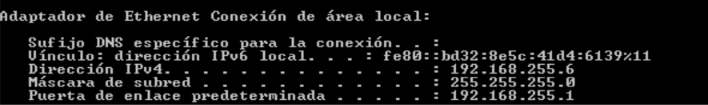
\includegraphics[width=0.85\textwidth]{Recursos/ip_WS.png}
    \caption{Configuración de red del servidor (\cod{192.168.255.6}).}
    \label{fig:ip-ws}
\end{figure}

\begin{figure}[H]
    \centering
    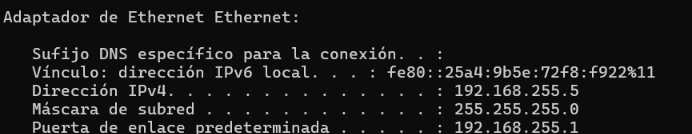
\includegraphics[width=0.85\textwidth]{Recursos/ip_pc_ladron.png}
    \caption{Configuración de red del equipo cliente (\cod{192.168.255.5}).}
    \label{fig:ip-w11}
\end{figure}

\subsubsection{Recurso compartido y extracción del documento}
El vector inicial es un recurso compartido SMB (\textit{Server Message Block})
del servidor. Para publicarlo, en las propiedades de la carpeta se activó
\textit{Compartir esta carpeta} con el nombre \cod{ConfidencialInfo}, se
asignaron los permisos de red al usuario autorizado y se comprobó que los
permisos locales NTFS le permitían el acceso, ya que Windows aplica siempre la
intersección más restrictiva de ambos. El comando \cod{net share} confirma la
publicación del recurso, asociado a la carpeta local \cod{C:\ConfidencialInfo}
(figura~\ref{fig:carpeta-compartida}).

\begin{figure}[H]
    \centering
    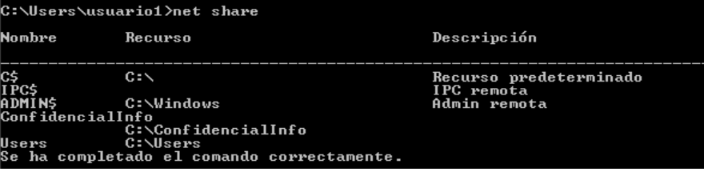
\includegraphics[width=0.85\textwidth]{Recursos/carpeta_compartida_WS.png}
    \caption{Recursos compartidos del servidor, con \cod{ConfidencialInfo}.}
    \label{fig:carpeta-compartida}
\end{figure}

Antes de la extracción se calculó la huella SHA-256 del fichero en el servidor
con \cod{certutil} (figura~\ref{fig:hash-ws}), para poder demostrar después
que la copia es idéntica al original.

\begin{figure}[H]
    \centering
    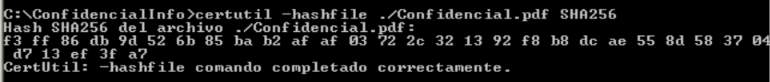
\includegraphics[width=0.85\textwidth]{Recursos/confidencial_en_WS_hash.png}
    \caption{Huella SHA-256 de \cod{Confidencial.pdf} en el servidor.}
    \label{fig:hash-ws}
\end{figure}

Desde el equipo cliente se accedió al recurso mediante su ruta UNC
(\textit{Universal Naming Convention}), sin asignar letra de unidad:

\begin{lstlisting}[style=terminal,breaklines=true]
explorer \\192.168.255.6\ConfidencialInfo
\end{lstlisting}

El fichero se copió a \cod{C:\Evidencias\Confidencial.pdf} en el equipo
cliente y se verificó con \cod{Get-FileHash} que su huella coincide con la del
servidor (figura~\ref{fig:hash-w11}).

\begin{figure}[H]
    \centering
    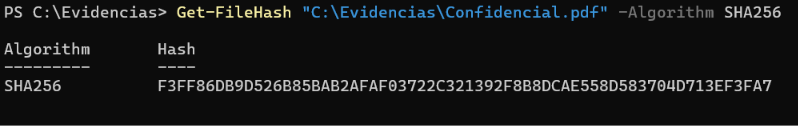
\includegraphics[width=0.85\textwidth]{Recursos/confidencial_en_Windows11_hash.png}
    \caption{Verificación con \cod{Get-FileHash} en \textit{Windows} 11 tras la
    extracción.}
    \label{fig:hash-w11}
\end{figure}

\subsubsection{Envío por correo electrónico}
Para no depender de servicios de terceros se empleó el servicio de correo
propio, con dos buzones: \cod{pepe@empresa.local} (origen, asociado al empleado)
y \cod{ana@empresa.local} (destino). Desde el equipo cliente se redactó un
mensaje de asunto <<Envío Confidencial>> dirigido a \cod{ana@empresa.local} con
\cod{Confidencial.pdf} como adjunto. El servidor lo procesó de forma interna y
lo depositó en el buzón de destino, sin que el tráfico saliera del laboratorio.
La figura~\ref{fig:correo-registrado} muestra el mensaje recibido en el
webmail: remitente, destinatario, fecha (martes 10 de noviembre de 2026,
18:26:34, hora \cod{+0100}) y el adjunto.

\begin{figure}[H]
    \centering
    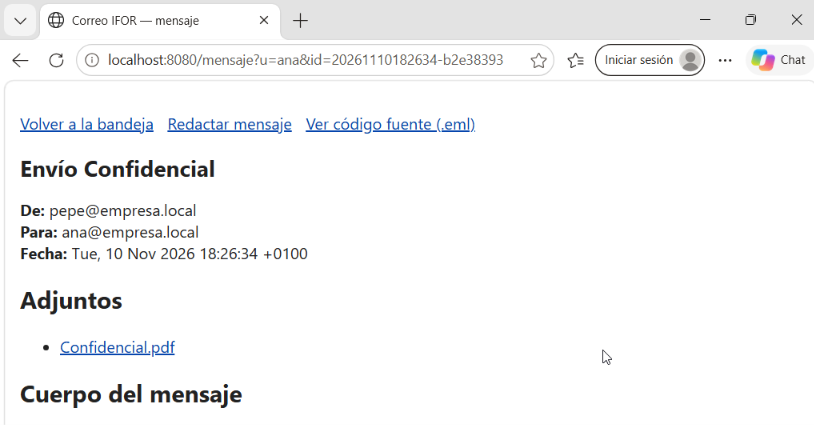
\includegraphics[width=0.85\textwidth]{Recursos/correo_registrado.png}
    \caption{Mensaje recibido en el buzón de \cod{ana@empresa.local}.}
    \label{fig:correo-registrado}
\end{figure}

% ---------------------------------------------------------------------
\subsection{Cadena de custodia}
\label{sec:correo-custodia}
Tras la simulación (10 de noviembre de 2026), la máquina virtual del equipo
cliente se apagó y su disco virtual, \cod{Maquina_Corrreo.vdi}, quedó como la
imagen de disco de este escenario. Conforme al supuesto del enunciado, el
director de la empresa, Jaime Diez Zurro, entrega al grupo esta imagen
\textbf{junto con la clave de recuperación de BitLocker}, sin la cual el
contenido del volumen del sistema no es legible (véase el apartado
\ref{sec:correo-bitlocker}). El peritaje de este escenario lo realiza
\PeritoDos, que es quien custodia el soporte.

Las fechas y horas de la tabla proceden de los metadatos del propio fichero
\cod{.vdi} en el equipo de análisis (última modificación, creación de la copia
y último acceso), de la creación de la captura con el \textit{hash} y de los
registros de la fase de análisis. No se precintó el soporte ni se calculó
ningún \textit{hash} antes del que se indica en la tabla, por lo que el estado
de la imagen queda fijado por ese cálculo. Todas las horas están en hora local
(CET, UTC+1).

\begin{table}[H]
\centering
\small
\renewcommand{\arraystretch}{1.3}
\begin{tabular}{@{}p{0.22\textwidth}p{0.13\textwidth}p{0.13\textwidth}p{0.43\textwidth}@{}}
\toprule
\textbf{Fecha y hora} & \textbf{Entrega} & \textbf{Recibe} & \textbf{Motivo y observaciones} \\
\midrule
10/11/2026, de 17:07 a 18:35 & -- & \PeritoDos &
Simulación de la fuga en las máquinas virtuales: configuración de red,
extracción desde el servidor y comprobación de huellas. El mensaje se envía a
las 18:26:34. \\
12/11/2026, 20:46:41 & -- & \PeritoDos &
Última modificación del disco virtual \cod{Maquina_Corrreo.vdi}: es la última
vez que la máquina virtual escribió en él. \\
12/11/2026, 20:52 & Jaime Diez Zurro (supuesto) & \PeritoDos &
Entrega de la imagen y de la clave de recuperación de BitLocker (protector
\cod{{04D7EFA5-4921-4EFD-8F65-7D2AAF4DF62A}}) al grupo para el peritaje, según
el supuesto del enunciado. Entrega simulada: el disco ya obraba en poder del
perito. La copia en la carpeta \cod{IFOR_CASO_CORREO} se creó a las 20:52:06. \\
12/11/2026, 20:59 & \PeritoDos & \PeritoDos (perito) &
Cálculo del primer \textit{hash} (SHA-256) de la imagen. \\
24/11/2026, hasta las 00:02 & \PeritoDos (perito) & \PeritoDos &
Se crea una copia de trabajo de la imagen y se comprueba que su \textit{hash}
es idéntico al del original. Después se cambia el identificador (UUID) de la
copia, para poder registrarla en \textit{VirtualBox}. \\
24/11/2026, de 00:05 a 00:48 & \PeritoDos (perito) & \PeritoDos &
Análisis en la máquina virtual \textit{Kali Linux}, con la copia de trabajo
conectada como disco inmutable. Cálculo del \textit{hash} del disco completo
al empezar y al terminar. \\
24/11/2026, 00:49 & \PeritoDos (perito) & \PeritoDos &
Recálculo de los \textit{hash} del original y de la copia. Custodia en el
equipo del perito, en la carpeta \cod{IFOR_CASO_CORREO}, sin modificar. \\
\bottomrule
\end{tabular}
\caption{Registro de custodia de la imagen del equipo cliente.}
\label{tab:correo-custodia}
\end{table}

% ---------------------------------------------------------------------
\subsection{Adquisición de la evidencia}
\label{sec:correo-adquisicion}

\subsubsection{Imagen utilizada}
Dado que el entorno completo se montó en \textit{VirtualBox}, el disco virtual
del equipo cliente puede utilizarse directamente como imagen del disco del
atacante interno. No se creó una imagen RAW con una herramienta de adquisición:
se trabaja sobre el propio \cod{.vdi}, que es un contenedor de disco virtual de
VirtualBox (no una copia bit a bit del soporte físico).

\begin{table}[H]
\centering
\small
\renewcommand{\arraystretch}{1.3}
\begin{tabular}{@{}p{0.34\textwidth}p{0.62\textwidth}@{}}
\toprule
\textbf{Parámetro} & \textbf{Valor} \\
\midrule
Fichero de imagen & \cod{Maquina_Corrreo.vdi} \\
Ubicación & \cod{C:\Users\hugop\Desktop\IFOR_CASO_CORREO} \\
Formato & Disco virtual VirtualBox (\cod{.vdi}) \\
Tamaño del fichero & 39.403.388.928 bytes (unos 36,7 GiB) \\
Tamaño del disco virtual & 85.899.345.920 bytes (80 GiB) \\
Última modificación & 12/11/2026, 20:46:41 \\
Creación de la copia & 12/11/2026, 20:52:06 \\
Copia de trabajo & \cod{copia_trabajo\Maquina_Corrreo_trabajo.vdi} \\
Equipo de análisis & \textit{Windows} 11 (compilación 26200) \\
Herramienta de cálculo & \cod{Get-FileHash} (\textit{PowerShell}) \\
\bottomrule
\end{tabular}
\caption{Parámetros de la imagen del equipo cliente.}
\label{tab:correo-imagen}
\end{table}

\subsubsection{Verificación de integridad}
Se calculó la huella SHA-256 de la imagen con la misma herramienta nativa de
\textit{Windows} que se había utilizado para el resto de ficheros
(figura~\ref{fig:correo-hash-imagen}). Se recalculó el 24 de noviembre de 2026,
al terminar el análisis, y el valor coincide con el de la captura, lo que
acredita que la imagen original no se modificó.

\begin{lstlisting}[style=terminal,breaklines=true]
Get-FileHash -Path "C:\Users\hugop\Desktop\IFOR_CASO_CORREO\Maquina_Corrreo.vdi" -Algorithm SHA256
SHA-256: 85EBDF723060F36E7E8EF4A6B848D85BFC2DB6B4B1597A51E13F676A193898A6
\end{lstlisting}

\begin{figure}[H]
    \centering
    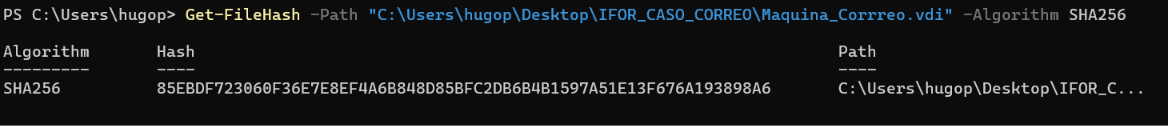
\includegraphics[width=0.85\textwidth]{Recursos/imagen_disco_correo.png}
    \caption{Huella SHA-256 de la imagen del disco del equipo cliente.}
    \label{fig:correo-hash-imagen}
\end{figure}

El análisis no se hace sobre el original, sino sobre una \textbf{copia de
trabajo}. Para poder registrarla en \textit{VirtualBox} (que no admite dos
discos con el mismo identificador) hubo que cambiarle el UUID, y ese cambio
modifica unos bytes de la cabecera del fichero. Por eso el \textit{hash} del
fichero de la copia ya no coincide con el del original. La comparación
relevante es la del \textbf{contenido}: el \textit{hash} de la copia justo
antes del cambio es idéntico al del original, y el \textit{hash} del disco
completo, visto desde \textit{Kali} (\cod{sha256sum /dev/sdb}), es el mismo al
empezar y al terminar el análisis (tabla~\ref{tab:correo-hashes}).

\begin{table}[H]
\centering
\footnotesize
\renewcommand{\arraystretch}{1.3}
\begin{tabular}{@{}p{0.34\textwidth}p{0.10\textwidth}p{0.50\textwidth}@{}}
\toprule
\textbf{Elemento} & \textbf{Alg.} & \textbf{Hash} \\
\midrule
Original \cod{.vdi} (12/11/2026) & SHA-256 & \cod{85EBDF723060F36E7E8EF4A6B848D85B}\newline
\cod{FC2DB6B4B1597A51E13F676A193898A6} \\
Original \cod{.vdi} (24/11/2026) & SHA-256 & \cod{85EBDF723060F36E7E8EF4A6B848D85B}\newline
\cod{FC2DB6B4B1597A51E13F676A193898A6} \\
Copia de trabajo, antes de cambiar el UUID & SHA-256 & \cod{85EBDF723060F36E7E8EF4A6B848D85B}\newline
\cod{FC2DB6B4B1597A51E13F676A193898A6} \\
Copia de trabajo, tras cambiar el UUID & SHA-256 & \cod{AE25F5C373F6834E914ADBBCA9776FDF}\newline
\cod{A6935678E946248054F4FB85F1CDE1E2} \\
Disco completo en \textit{Kali} (inicio) & SHA-256 & \cod{d97ac1ddf9f650ffb35b1ea757e5756a}\newline
\cod{29582980fcb006843321d78a2936e714} \\
Disco completo en \textit{Kali} (final) & SHA-256 & \cod{d97ac1ddf9f650ffb35b1ea757e5756a}\newline
\cod{29582980fcb006843321d78a2936e714} \\
\bottomrule
\end{tabular}
\caption{Verificación de integridad de la imagen y de la copia de trabajo.}
\label{tab:correo-hashes}
\end{table}

\noindent\textbf{Importante.} La imagen original se conserva sin modificar, con
su \textit{hash} registrado en la cadena de custodia. Todo el examen se hace
sobre la copia, sin arrancar nunca la máquina virtual original, porque al
iniciarse modificaría el \cod{.vdi}.

\subsubsection{Entorno y herramientas de análisis}
\label{sec:correo-herramientas}
El análisis se realizó en la máquina virtual \textit{Kali Linux} 2025.3
(núcleo 6.12.38), a la que se conectó la copia de trabajo como disco
\textbf{inmutable}: \textit{VirtualBox} no permite disco duro de solo lectura,
y el modo inmutable envía cualquier escritura a un fichero aparte sin tocar la
copia. Además, dentro de \textit{Kali} se activó el bloqueo de escritura del
disco (\cod{blockdev --setro}, resultado \cod{1}). Se emplearon las
herramientas de la tabla~\ref{tab:correo-herramientas}, todas estándar y
libres. Las órdenes y las salidas completas se conservan en la carpeta de
evidencias.

\begin{table}[H]
\centering
\small
\renewcommand{\arraystretch}{1.3}
\begin{tabular}{@{}p{0.24\textwidth}p{0.14\textwidth}p{0.54\textwidth}@{}}
\toprule
\textbf{Herramienta} & \textbf{Versión} & \textbf{Uso} \\
\midrule
\cod{fdisk}, \cod{mmls} & \textit{TSK} 4.12.1 & Tabla de particiones del disco \\
\cod{cryptsetup bitlkDump} & 2.8.1 & Lectura de los metadatos de BitLocker \\
\cod{dislocker} & 0.7.4 & Descifrado de BitLocker en solo lectura con la clave de recuperación \\
\cod{fsstat}, \cod{fls}, \cod{istat}, \cod{icat} & \textit{TSK} 4.12.1 & Examen del sistema de ficheros NTFS: listado, metadatos y extracción \\
\cod{mactime} & \textit{TSK} 4.12.1 & Línea temporal \\
\cod{md5sum}, \cod{sha1sum}, \cod{sha256sum} & coreutils & Huellas de integridad \\
\bottomrule
\end{tabular}
\caption{Herramientas utilizadas en \textit{Kali Linux}.}
\label{tab:correo-herramientas}
\end{table}

\subsubsection{Estructura del disco y cifrado BitLocker}
\label{sec:correo-bitlocker}
El disco usa tabla de particiones GPT con cuatro particiones
(tabla~\ref{tab:correo-particiones}). La partición del sistema (\cod{C:}) está
\textbf{cifrada con BitLocker}: su primer sector no contiene la firma de NTFS
sino la de BitLocker (\cod{-FVE-FS-}), por lo que sin la clave el contenido no
es legible. Es lo habitual en equipos con \textit{Windows} 11, que activa el
cifrado de dispositivo de forma predeterminada.

\begin{table}[H]
\centering
\small
\renewcommand{\arraystretch}{1.3}
\begin{tabular}{@{}p{0.07\textwidth}p{0.18\textwidth}p{0.20\textwidth}p{0.45\textwidth}@{}}
\toprule
\textbf{N.º} & \textbf{Sector inicial} & \textbf{Sectores} & \textbf{Contenido} \\
\midrule
1 & 2.048 & 409.600 & Partición del sistema EFI (200 MB) \\
2 & 411.648 & 32.768 & Reservada de Microsoft (16 MB) \\
3 & 444.416 & 165.470.208 & Volumen \cod{C:}, cifrado con BitLocker (78,9 GB) \\
4 & 165.914.624 & 1.853.440 & Entorno de recuperación de Windows (905 MB) \\
\bottomrule
\end{tabular}
\caption{Particiones del disco del equipo cliente (sectores de 512 bytes).}
\label{tab:correo-particiones}
\end{table}

Los metadatos de BitLocker (figura~\ref{fig:correo-kali-bitlocker}) indican
que el volumen se creó el 9 de noviembre de 2026, con la descripción
\cod{DESKTOP-DI359N9 C: 09/11/2026}, y que usa el cifrado \textbf{AES-XTS de
128 bits}. Tiene dos protectores de la clave maestra: una \textit{clave de
recuperación} (identificador \cod{04d7efa5-4921-4efd-8f65-7d2aaf4df62a}) y una
\textit{clave en claro}. Esta última es la que Windows deja cuando el cifrado
está \textbf{suspendido}: en ese estado la clave queda accesible para el
propio sistema.

\begin{figure}[H]
    \centering
    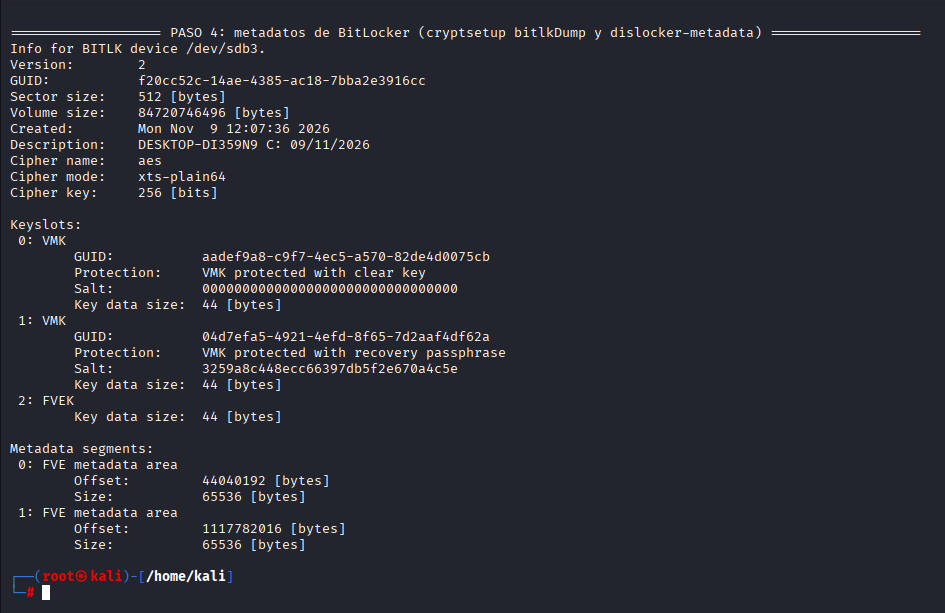
\includegraphics[width=0.85\textwidth]{Recursos/correo_kali_bitlocker.png}
    \caption{Metadatos de BitLocker del volumen \cod{C:} (\cod{cryptsetup bitlkDump}).}
    \label{fig:correo-kali-bitlocker}
\end{figure}

Conforme al supuesto del enunciado, la clave de recuperación la facilita el
director de la empresa junto con el equipo (véase la
tabla~\ref{tab:correo-custodia}). Con ella se descifró el volumen en solo
lectura:

\begin{lstlisting}[style=terminal,breaklines=true]
dislocker -V /dev/sdb3 -p<clave de recuperacion> -r -- /mnt/bitlocker
\end{lstlisting}

\textit{dislocker} presenta el volumen en claro como un fichero
(\cod{dislocker-file}) que \textit{The Sleuth Kit} reconoce como NTFS, con
259.073 entradas en la \cod{\$MFT} (figura~\ref{fig:correo-kali-dislocker}).
Se probó antes con \cod{cryptsetup bitlkOpen}, pero esta herramienta no
admite volúmenes con la clave en claro (cifrado suspendido), por lo que se
utilizó \textit{dislocker}. La clave de recuperación no se reproduce en este
informe.

\begin{figure}[H]
    \centering
    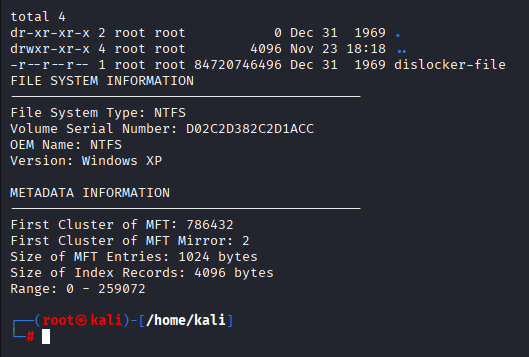
\includegraphics[width=0.6\textwidth]{Recursos/correo_kali_dislocker.png}
    \caption{Volumen descifrado y reconocido como NTFS (\cod{fsstat}).}
    \label{fig:correo-kali-dislocker}
\end{figure}

% ---------------------------------------------------------------------
\subsection{Informe de pruebas}
\label{sec:correo-analisis}

En el volumen \cod{C:} descifrado se localizó el servidor de correo del grupo,
en \cod{C:\Users\hugop\Downloads\IFOR_P2-main\IFOR_P2-main\servidor}, junto
con los tres elementos que genera por cada envío (mensaje, adjunto y registro).
Se obtuvo el listado de ficheros con \cod{fls}, se consultaron sus metadatos con
\cod{istat} y se extrajeron con \cod{icat}, calculando su MD5, SHA-1 y SHA-256.

\textbf{Nota sobre las horas.} Las marcas temporales de NTFS están en UTC.
\cod{istat} las muestra en la zona horaria de \textit{Kali} (EST, UTC$-$5) y
\cod{mactime} se ejecutó en UTC. En este informe se convierten a hora local
(CET, UTC+1): 17:26:34 UTC (12:26:34 EST) son las 18:26:34 de la hora del
mensaje.

\subsubsection{Prueba 1: mensaje \cod{.eml}}
Se trata del fichero
\cod{servidor\buzones\ana\mensajes\20261110182634-b2e38393.eml} (entrada 226668 de
la \cod{\$MFT}, activa, 920 bytes). Su contenido, sin alterar, es:

\begin{lstlisting}[style=terminal,basicstyle=\ttfamily\footnotesize,breaklines=true]
Received: from webmail (127.0.0.1)
	by empresa.local (servidor IFOR) with HTTP;
	Tue, 10 Nov 2026 18:26:34 +0100
From: pepe@empresa.local
To: ana@empresa.local
Subject: =?utf-8?q?Env=C3=ADo?= Confidencial
Date: Tue, 10 Nov 2026 18:26:34 +0100
Message-ID: <179433159411.4376.15980925307143410306@DESKTOP-DI359N9>
Content-Type: multipart/mixed; boundary="===============1681336223577990369=="
...
Content-Type: application/pdf
Content-Transfer-Encoding: base64
Content-Disposition: attachment; filename="Confidencial.pdf"
\end{lstlisting}

\begin{table}[H]
\centering
\small
\renewcommand{\arraystretch}{1.3}
\begin{tabular}{@{}p{0.28\textwidth}p{0.68\textwidth}@{}}
\toprule
\textbf{Campo} & \textbf{Valor} \\
\midrule
Remitente (\cod{From}) & \cod{pepe@empresa.local} \\
Destinatario (\cod{To}) & \cod{ana@empresa.local} \\
Asunto & Envío Confidencial \\
Fecha (\cod{Date}) & Tue, 10 Nov 2026 18:26:34 +0100 \\
\cod{Received} & de \cod{webmail (127.0.0.1)}, por \cod{empresa.local} (servidor IFOR), con \cod{HTTP} \\
Identificador del mensaje & \cod{<179433159411.4376.}\newline\cod{15980925307143410306@DESKTOP-DI359N9>} \\
Adjunto & \cod{Confidencial.pdf} (\cod{application/pdf}, base64) \\
SHA-256 del \cod{.eml} & \cod{1446aec75726e0bc745898a4055316e6}\newline
\cod{65cf52840236b520b16c3c315c8b2fd9} \\
\bottomrule
\end{tabular}
\caption{Cabeceras y huella del mensaje recuperado.}
\label{tab:correo-cabeceras}
\end{table}

La cabecera \cod{Received} indica que el mensaje entró por el \textit{webmail}
desde la dirección local \cod{127.0.0.1}, es decir, desde la propia máquina
donde se ejecuta el servidor. La hora de la cabecera \cod{Date} coincide con la
captura del \textit{webmail} (figura~\ref{fig:correo-registrado}).

\begin{figure}[H]
    \centering
    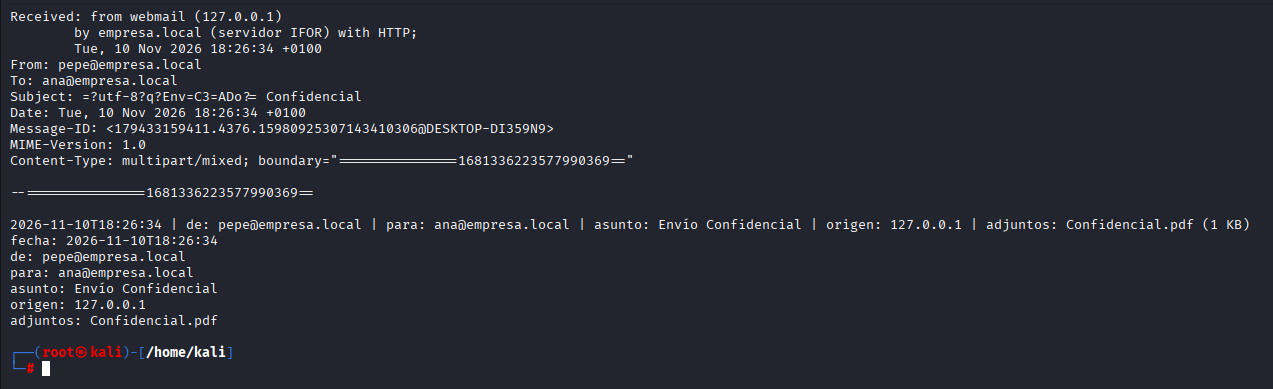
\includegraphics[width=0.9\textwidth]{Recursos/correo_kali_eml_logs.png}
    \caption{Mensaje, registro de envíos y fichero \cod{envio.txt} extraídos.}
    \label{fig:correo-kali-eml}
\end{figure}

\subsubsection{Prueba 2: adjunto y comparación con el original}
El adjunto aparece en tres puntos de la imagen (tabla~\ref{tab:correo-adjuntos}):
decodificado del propio \cod{.eml} (el 	extit{Base64} se decodificó con 	extit{PowerShell}), extraído por el servidor al buzón de
destino y guardado en la carpeta de copias de envío. A ello se suma la copia de
origen en el equipo cliente, \cod{C:\Evidencias\Confidencial.pdf}. Los cuatro
ficheros son de 103 bytes y tienen el \textbf{mismo SHA-256 que el original}
calculado en el servidor (\cod{f3ff86db\ldots3fa7}). Su contenido es un texto
breve en el que el gerente de la empresa indica que se trata de información
confidencial, igual que en los demás escenarios.

\begin{table}[H]
\centering
\footnotesize
\renewcommand{\arraystretch}{1.3}
\begin{tabular}{@{}p{0.30\textwidth}p{0.66\textwidth}@{}}
\toprule
\textbf{Fichero (entrada \cod{\$MFT})} & \textbf{SHA-256} \\
\midrule
Original en el servidor (certutil) & \cod{f3ff86db9d526b85bab2afaf03722c32}\newline
\cod{1392f8b8dcae558d583704d713ef3fa7} \\
Adjunto decodificado del \cod{.eml} & \cod{f3ff86db9d526b85bab2afaf03722c32}\newline
\cod{1392f8b8dcae558d583704d713ef3fa7} \\
\cod{buzones\ana\adjuntos\...} (226671) & \cod{f3ff86db9d526b85bab2afaf03722c32}\newline
\cod{1392f8b8dcae558d583704d713ef3fa7} \\
\cod{adjuntos_enviados\...} (226675) & \cod{f3ff86db9d526b85bab2afaf03722c32}\newline
\cod{1392f8b8dcae558d583704d713ef3fa7} \\
\cod{C:\Evidencias\Confidencial.pdf} (234421) & \cod{f3ff86db9d526b85bab2afaf03722c32}\newline
\cod{1392f8b8dcae558d583704d713ef3fa7} \\
\bottomrule
\end{tabular}
\caption{Comparación del adjunto con el original. Coinciden todos.}
\label{tab:correo-adjuntos}
\end{table}

El MD5 del adjunto, \cod{4c9283480e5692410e177df58323e732}, coincide también
con el que \textit{Autopsy} muestra para el fichero del escenario de
\textit{Dropbox}, lo que confirma que es el mismo documento en los tres
escenarios.

\begin{figure}[H]
    \centering
    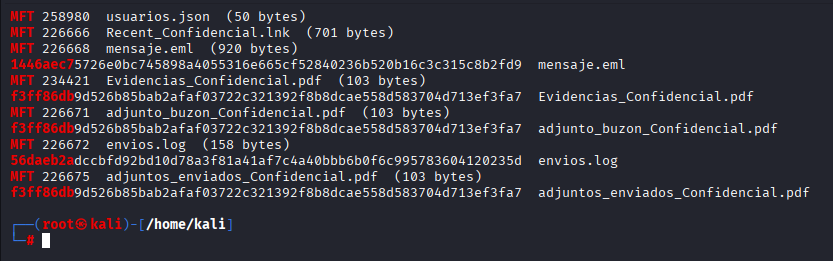
\includegraphics[width=0.9\textwidth]{Recursos/correo_kali_hashes.png}
    \caption{Huellas calculadas en \textit{Kali} de los ficheros extraídos.}
    \label{fig:correo-kali-hashes}
\end{figure}

\subsubsection{Prueba 3: registro de envíos}
El fichero \cod{servidor\logs\envios.log} (entrada 226672, 158 bytes, SHA-256
\cod{56daeb2adccbfd92bd10d78a3f81a41af7c4a40bbb6b0f6c995783604120235d})
contiene una única línea:

\begin{lstlisting}[style=terminal,basicstyle=\ttfamily\footnotesize,breaklines=true]
2026-11-10T18:26:34 | de: pepe@empresa.local | para: ana@empresa.local | asunto: Envío Confidencial | origen: 127.0.0.1 | adjuntos: Confidencial.pdf (1 KB)
\end{lstlisting}

Remitente, destinatario, asunto, adjunto, origen y hora \textbf{coinciden} con
el \cod{.eml}: la hora del registro es la de la cabecera \cod{Date} y el origen
es el mismo (\cod{127.0.0.1}). El fichero \cod{usuarios.json} (entrada 258980)
confirma que los únicos buzones del servidor son \cod{ana} y \cod{pepe}.

\subsubsection{Prueba 4: ficheros complementarios}
Junto al envío existen otros ficheros que apoyan el relato:

\begin{itemize}
  \item \textbf{\cod{envio.txt}} (entrada 226676, 153 bytes, SHA-256
        \cod{22cb3a21\ldots15d3}), en la carpeta de copias de envío
        \cod{adjuntos_enviados\2026-11-10_18-26-34_a29091c4}. Repite fecha,
        remitente, destinatario, asunto, origen (\cod{127.0.0.1}) y adjunto,
        y coincide con el \cod{.eml} y el registro.
  \item \textbf{Acceso reciente} \cod{Recent\Confidencial.lnk} (entrada
        226666, 701 bytes), creado a las 18:26:31 locales, tres segundos antes
        del envío. Apunta a \cod{C:\Evidencias\Confidencial.pdf} y al equipo
        \cod{desktop-di359n9}: indica que el fichero se abrió desde esa ruta
        justo antes de enviarlo.
  \item \textbf{Marca \cod{Zone.Identifier}} del fichero
        \cod{C:\Evidencias\Confidencial.pdf} (flujo alternativo de NTFS,
        26 bytes), con el contenido \cod{[ZoneTransfer] ZoneId=3}. Es un
        indicador que Windows añade a los ficheros recibidos por vías
        externas; se hace constar como hallazgo, sin extraer más conclusiones.
\end{itemize}

\subsubsection{Prueba 5: marcas temporales del sistema de ficheros}
La tabla~\ref{tab:correo-fechas} reúne las fechas de los ficheros implicados,
tomadas del atributo \cod{\$STANDARD\_INFORMATION} con \cod{istat} y
contrastadas con la línea temporal de \cod{mactime}. Los atributos
\cod{\$FILE\_NAME} de todos ellos son coherentes con las fechas de creación.

\begin{table}[H]
\centering
\footnotesize
\renewcommand{\arraystretch}{1.3}
\begin{tabular}{@{}p{0.36\textwidth}p{0.20\textwidth}p{0.20\textwidth}p{0.17\textwidth}@{}}
\toprule
\textbf{Fichero} & \textbf{Creación (UTC)} & \textbf{Modificación (UTC)} & \textbf{Acceso (UTC)} \\
\midrule
\cod{Evidencias\Confidencial.pdf} & 10/11 17:20:19 & 28/10 18:11:08 & 10/11 17:26:34 \\
\cod{Recent\Confidencial.lnk} & 10/11 17:26:31 & 10/11 17:26:31 & 10/11 17:26:31 \\
Mensaje \cod{.eml} & 10/11 17:26:34 & 10/11 17:26:36 & 10/11 17:26:59 \\
Adjunto en el buzón & 10/11 17:26:34 & 10/11 17:26:34 & 10/11 17:26:36 \\
\cod{envios.log} & 10/11 17:26:34 & 10/11 17:26:34 & 10/11 17:26:34 \\
Copia en \cod{adjuntos_enviados} & 10/11 17:26:34 & 10/11 17:26:34 & 10/11 17:26:36 \\
\bottomrule
\end{tabular}
\caption{Marcas temporales de los ficheros del envío (hora UTC).}
\label{tab:correo-fechas}
\end{table}

La fecha de modificación de \cod{Evidencias\Confidencial.pdf}
(28/10/2026, 18:11:08 UTC, es decir 19:11:08 en hora local) es la del fichero
original en el servidor, que se conserva al copiarlo; su creación (17:20:19)
es el momento de la copia al equipo cliente. La fecha de modificación del
\cod{.eml} es 2,4 segundos posterior a la de creación; no se ha podido
determinar la causa, aunque su contenido es coherente con el registro.

\subsubsection{Línea temporal reconstruida}
\begin{table}[H]
\centering
\small
\renewcommand{\arraystretch}{1.3}
\begin{tabular}{@{}p{0.20\textwidth}p{0.45\textwidth}p{0.27\textwidth}@{}}
\toprule
\textbf{Hora local} & \textbf{Hecho} & \textbf{Fuente} \\
\midrule
09/11/2026, 20:33 & Despliegue del servidor de correo en el equipo cliente & Fechas de la carpeta \cod{servidor} \\
10/11/2026, 18:20:19 & Copia de \cod{Confidencial.pdf} a \cod{C:\Evidencias} & Creación del fichero \\
10/11/2026, 18:23:34 & Creación de los buzones y del registro & \cod{usuarios.json}, \cod{logs} \\
10/11/2026, 18:26:31 & Apertura de \cod{Confidencial.pdf} & Acceso reciente (\cod{.lnk}) \\
10/11/2026, 18:26:34 & Envío de \cod{pepe@empresa.local} a \cod{ana@empresa.local} con el adjunto & \cod{.eml}, \cod{envios.log}, \cod{envio.txt} \\
12/11/2026, 20:46:41 & Última escritura en el disco virtual & Metadatos del \cod{.vdi} \\
\bottomrule
\end{tabular}
\caption{Línea temporal del escenario de correo.}
\label{tab:correo-linea}
\end{table}

El servidor de correo se ejecutó en la propia máquina del equipo cliente (el
\cod{Received} indica origen \cod{127.0.0.1}), de modo que el envío por
\textit{webmail} y la recepción en el buzón de \cod{ana} quedan registrados en
el mismo disco.

% ---------------------------------------------------------------------
\subsection{Conclusiones}
La imagen del equipo cliente, descifrada en solo lectura con la clave de
recuperación de BitLocker, contiene la prueba del envío. El mensaje con
\cod{Confidencial.pdf} adjunto se envió el 10 de noviembre de 2026 a las
18:26:34 desde \cod{pepe@empresa.local} hacia \cod{ana@empresa.local} a través
del \textit{webmail}, tras copiar el fichero desde el recurso compartido del
servidor al equipo cliente. El \cod{.eml}, el adjunto extraído, el registro
\cod{envios.log} y el fichero \cod{envio.txt} coinciden entre sí, y el SHA-256
del adjunto es idéntico al del original, por lo que el documento enviado es el
mismo que el del servidor.

Las limitaciones son las siguientes. El servicio de correo no implementa
autenticación, por lo que los registros SMTP por sí solos no permiten atribuir
el envío a una persona concreta; solo se acredita que se hizo desde la máquina
del equipo cliente. Además, la imagen es un disco virtual y no una copia bit a
bit de un soporte físico, estaba cifrada con BitLocker en estado suspendido, y
se analizó una copia de trabajo cuyo UUID fue modificado, lo que impide que el
\textit{hash} del fichero coincida con el del original (el contenido sí es el
mismo, según el \textit{hash} del disco completo). Por último, el soporte
estuvo sin precinto ni \textit{hash} hasta el 12 de noviembre de 2026, de modo
que su estado queda fijado desde ese momento.


\subsection{Sobre Dropbox}
	\subsection{Escenario 2: fuga mediante DropBox}


\subsection{Sobre USB }
	%% =====================================================================
% Capítulo: Escenario 3 -- fuga de información mediante dispositivo USB
% Esqueleto: los apartados marcados con TODO se rellenan al ejecutar
% cada paso en el laboratorio (hashes, fechas, capturas y resultados).
%
% Solo usa lo que define styles/mistilo.sty:
%   - listados:  style=terminal
%   - avisos:    entorno aviso
%   - tablas:    booktabs + caption
% =====================================================================

% Código en línea (admite _, $, ^, {}, <, > ... sin escapar). Se vuelve a
% declarar por si este capítulo se compila solo con \includeonly.
\providecommand{\cod}[1]{\texttt{\detokenize{#1}}}

\subsection{Escenario 3: fuga de información mediante dispositivo USB}
\label{cap:usb}

En este capítulo se documenta el tercero de los escenarios del enunciado: la
fuga del fichero \cod{Confidencial.pdf} del \textit{Windows Server} 2008 hacia un
dispositivo USB. En este caso el dispositivo está en nuestro poder, pero el
fichero ha sido \textbf{borrado}, de modo que el trabajo consiste en adquirir
una imagen forense del soporte sin modificarlo, recuperar el fichero y
mantener la cadena de custodia.

% ---------------------------------------------------------------------
\subsection{Planteamiento y alcance}
% TODO: resumir en 2-3 párrafos qué se pide y qué queda fuera.

\begin{itemize}
  \item \textbf{Origen:} \cod{Confidencial.pdf} en el \textit{Windows Server}
        2008 configurado en la entrega anterior.
  \item \textbf{Soporte a analizar:} un dispositivo USB que se nos entrega
        con el fichero ya borrado.
  \item \textbf{Entregable:} imagen forense del USB, recuperación del fichero,
        cadena de custodia y conclusiones.
  \item \textbf{Formato de la imagen:} el soporte USB se adquiere en formato
        \textbf{RAW} (copia bit a bit, sin comprimir); el resto de imágenes
        del trabajo sí pueden ir comprimidas.
\end{itemize}

% ---------------------------------------------------------------------
\subsection{Preparación del escenario}
% TODO: describir cómo se simula la fuga. Todo con fecha y hora.

\subsubsection{Entorno de trabajo}
Para el desarrollo de este escenario se ha utilizado la máquina virtual
\cod{IFOR-WS-2008}, con \textit{Windows Server} 2008, importada en VirtualBox a
partir de la imagen OVA común del grupo. Para permitir el acceso a dispositivos USB desde la máquina
virtual se ha instalado el \textit{Extension Pack} de VirtualBox, versión
7.2.18.

El fichero original, \cod{Confidencial.pdf}, se encuentra en
\cod{C:\Empresa\ConfidencialInfo}, tiene un tamaño de 103 bytes y fue creado el
28/10/2026 a las 19:10:00 (última modificación a las 19:11:08). Su contenido es
un texto breve en el que el gerente de la empresa indica que se trata de
información confidencial. Antes de iniciar la simulación se calculó su huella
SHA-256, que se utilizará como referencia en la verificación final:

\begin{lstlisting}[style=terminal,breaklines=true]
SHA-256 (Confidencial.pdf): f3ff86db9d526b85bab2afaf03722c321392f8b8dcae558d583704d713ef3fa7
\end{lstlisting}

\subsubsection{Dispositivo USB utilizado}

\begin{table}[H]
\centering
\small
\renewcommand{\arraystretch}{1.3}
\begin{tabular}{@{}p{0.32\textwidth}p{0.64\textwidth}@{}}
\toprule
\textbf{Característica} & \textbf{Valor} \\
\midrule
Marca y modelo & General UDisk \\
Capacidad & 3,75 GB \\
Número de serie & \cod{2504021555480511776507} \\
Sistema de ficheros & NTFS \\
\bottomrule
\end{tabular}
\caption{Ficha del dispositivo USB.}
\label{tab:usb-ficha}
\end{table}

Para la simulación se ha utilizado un pendrive vacío, que originalmente estaba
formateado en FAT32 con tabla de particiones MBR (figura~\ref{fig:usb-inicial}).
Desde la máquina virtual se le dio formato rápido en NTFS mediante
\cod{format E: /FS:NTFS /Q} (figura~\ref{fig:usb-formato}), quedando una única
unidad de 3,75 GB sin contenido (figura~\ref{fig:usb-final}).

\begin{figure}[H]
\centering
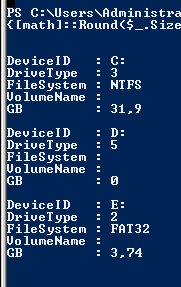
\includegraphics[width=0.3\textwidth]{Recursos/usb_estado_inicial.png}
\caption{Estado inicial del dispositivo: unidad \cod{E:} extraíble en FAT32.}
\label{fig:usb-inicial}
\end{figure}

\begin{figure}[H]
\centering
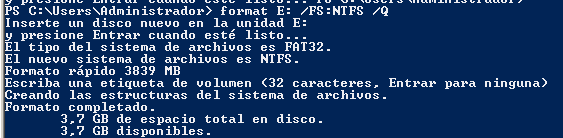
\includegraphics[width=0.8\textwidth]{Recursos/usb_formato_ntfs.png}
\caption{Formato rápido de la unidad \cod{E:} en NTFS.}
\label{fig:usb-formato}
\end{figure}

\begin{figure}[H]
\centering
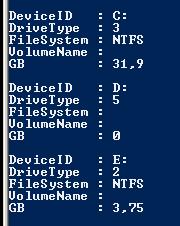
\includegraphics[width=0.3\textwidth]{Recursos/usb_estado_final.png}
\caption{Estado final del dispositivo: unidad \cod{E:} en NTFS.}
\label{fig:usb-final}
\end{figure}

\subsubsection{Simulación de la fuga}
La fuga se simuló desde la propia máquina virtual el jueves 12 de noviembre de
2026 (hora de la máquina virtual), siguiendo estos pasos:

\begin{enumerate}
  \item A las 16:19:56 se copió \cod{Confidencial.pdf} desde
        \cod{C:\Empresa\ConfidencialInfo} a la unidad \cod{E:} del dispositivo
        USB (figura~\ref{fig:usb-copia}).
  \item Se comprobó que la copia era idéntica al original: su huella SHA-256
        coincide con la calculada previamente
        (figura~\ref{fig:usb-hash-copia}).
  \item A las 16:21:25 se borró el fichero del USB con \cod{Remove-Item}. Al
        tratarse de un dispositivo extraíble, que no dispone de papelera de
        reciclaje, el borrado es directo (figura~\ref{fig:usb-borrado}).
  \item A las 16:22:43 se expulsó el dispositivo mediante la opción <<Quitar
        hardware de forma segura>> y se desconectó de la máquina virtual.
\end{enumerate}

\begin{figure}[H]
\centering
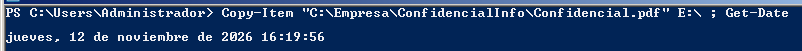
\includegraphics[width=0.8\textwidth]{Recursos/usb_copia.png}
\caption{Copia de \cod{Confidencial.pdf} al USB (16:19:56).}
\label{fig:usb-copia}
\end{figure}

\begin{figure}[H]
\centering
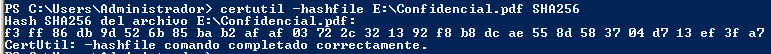
\includegraphics[width=0.8\textwidth]{Recursos/usb_hash_copia.png}
\caption{Verificación de la huella SHA-256 de la copia en el USB.}
\label{fig:usb-hash-copia}
\end{figure}

\begin{figure}[H]
\centering
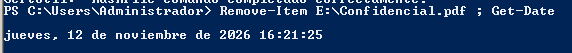
\includegraphics[width=0.8\textwidth]{Recursos/usb_borrado.png}
\caption{Borrado del fichero del USB (16:21:25).}
\label{fig:usb-borrado}
\end{figure}



\newpage

\section{CONCLUSIONES}

En opinión de este perito\ldots\ldots\ldots\ldots

A juicio de este perito \ldots\ldots\ldots

A juicio de este perito \ldots\ldots

Una vez analizado \ldots\ldots\ldots

Lo que hago constar como perito en este dictamen, salvo mejor opinión a la que me someto, para lo cual, pondré a disposición de quien lo solicite, todos los medios utilizados para llegar a las conclusiones a las que he llegado.

Emito por tanto este dictamen extendido en \NumFolios\ folios, según mi leal saber y entender, prometiendo que en el momento de emitirlo, he dicho la verdad y he actuado con la mayor objetividad posible, tomando en consideración tanto lo que pueda favorecer como lo que sea susceptible de causar perjuicio a cualquiera de las partes.

\vspace{2.2cm}
\begin{flushright}
    \begin{minipage}{0.55\textwidth}
        \centering
        \rule{6cm}{0.4pt} \\[0.2cm]
        \textbf{Nombre Apellidos y Firma del perito} \\
        \PeritoNombre \\
        Colegiado n.\textsuperscript{o} \NumColegiado \\[0.4cm]
        En \CiudadFirma\ a \FechaFirma.
    \end{minipage}
\end{flushright}

\newpage

\section{Sobre la metodología empleada en la elaboración del presente informe pericial}

Para la elaboración de este dictamen, la metodología empleada ha sido la siguiente:

\begin{itemize}[leftmargin=1.5em]
    \item Revisión de la documentación entregada por \Cliente.
    \item Revisión de documentos etc etc.
    \item Revisión del software \ldots\ldots
    \item Estudio y documentación sobre \ldots\ldots\ldots
    \item Redacción del presente informe.
\end{itemize}

\newpage

\section{BIBLIOGRAFÍA Y REFERENCIAS A CONSULTAR}

Para la elaboración de este dictamen, este perito se ha basado además de en sus conocimientos, en una serie de referencias bibliográficas sobre Ingeniería Informática entre las que se encuentran:

\begin{itemize}[leftmargin=1.5em]
    \item Libro 1
    \item Libro 2
    \item Revista
    \item Artículo de internet.
\end{itemize}

\newpage

% ------------------------------------------------------------------------------
% BLOQUE DE ANEXOS Y EVIDENCIAS (CARPETA: anexos/)
% ------------------------------------------------------------------------------
\appendix
\renewcommand{\thesection}{\Alph{section}}

\section*{EVIDENCIAS}
\addcontentsline{toc}{section}{EVIDENCIAS}

Para la realización de este informe se han utilizado como evidencias\ldots\ldots\ldots

Se adjuntan como evidencias los ficheros implicados en el caso, extraídos en un disco USB con número de serie: \texttt{5\&1D45E55A\&0\&6}, referenciados a continuación con su correspondiente código de autentificación hash de tipo SHA-1:

\begin{itemize}[leftmargin=1.5em]
    \item Fichero en formato PDF que contiene todos los SMS con el número 99999999: \\
    \texttt{< D:\textbackslash xxxxxxxxxxx.pdf >} \\
    \textbf{SHA-1:} \texttt{7F281355ECD8F9D6834B9484B5B18362E758D66B}

    \item Fichero en formato RAR con la copia completa del iPhone: \\
    \texttt{< D:\textbackslash jhgjhgjhgjkhgd.rar >} \\
    \textbf{SHA-1:} \texttt{EBF0011BDEE1B0D5D40ACDFD3379AF1318489323}
\end{itemize}

Durante la realización de este informe se han generado como evidencias\ldots\ldots\ldots


% Descomenta las siguientes líneas si deseas incluir un segundo anexo con capturas y trazas:
% \newpage
% \section{Capturas técnicas y trazas de registro (Plantilla opcional)}

% Este fichero sirve de modelo para añadir anexos documentales adicionales.
% Las imágenes depositadas en la carpeta resources/ pueden invocarse directamente por su nombre:

En el presente anexo se adjuntan las capturas de pantalla y extractos técnicos obtenidos durante el análisis forense.

% Ejemplo de inserción de figura desde resources/:
% \begin{figure}[htbp]
%     \centering
%     \includegraphics[width=0.85\textwidth]{captura_evidencia_01.png}
%     \caption{Captura del registro de eventos analizado.}
%     \label{fig:evidencia_01}
% \end{figure}


\end{document}
